\section{Evaluation}
\label{sect:evaluation}

We have implemented a \sysname prototype as a Django web application
that features the REST API presented in Section~\ref{sect:fairtest}.
We evaluated our prototype by using it to uncover {\it privacy bugs}
in the pricing policy of the ``Staples Inc.'', as described by the
Wall Street Journal in 2012. We sought answer to the following three
questions:

\begin{enumerate}
  \item[{\bf Q1}] Can \sysname uncover any {\em privacy bugs} in the
    pricing policy of the ``Staples Inc.'' online store?
  \item[{\bf Q2}] What is the impact of any privacy bugs in the outputs
    shown to users?
  \item[{\bf Q3}] What is the dependency of privacy bugs on the 
    pricing policy? Is the impact of {\em privacy bugs} constant,
    or varies for diffent pricing policies?
\end{enumerate}

\subsection{\normalsize Methodology}
Our experimental evaluation of \sysname consists of the following three steps:

\begin{enumerate}
  \item
  Generate one million synthetic users that are spread accross the
  areas corresponding to 40,000 US zip-codes. These synthetic users
  have four attributes: zip-code, race, sex, and income, and match
  the demographic characteristics of the US population, according to
  the US Census Bureau~\cite{CensusBureau}, as of May 3, 2014.
  \footnote{
    The infrastructure necessary for generating syntetic users is
    provided by a project of the ``Advanced Distributed Systems'' course,
    tought by professor Roxana Geambasu, Spring 2015. The developers of the
    project are Z. Zhou, Z. Wan, and X. Ma.
  }

  \item
  Use the users generated in Step 1 to simulate one million user-visits on
  an online store with a pricing engine that implements the pricing policy of
  the ``Staples Inc.'' online store. After each visit, register to \sysname
  the respective synthetic user along with the received output.

  \item
  Query \sysname's web interface to uncover any strong correlation between
  outputs and protected user attributes, i.e., race, income, and sex.
\end{enumerate}

Since user-attributes match the demographics of the US popation,
race, sex, and income are assigned values that depend on the zip-code. Because
the later defines the area in which a user lives. In other words, user's race,
sex, and income correlate with user's zip-code, but not amongst each other.
Each user has
one of the following races:  (i) ``White'', (ii) ``Hispanic'', (iii) ``African
American'', (iv) ``Indian or Alaskan'', (v) ``Asian'', (vi) ``Pacific
Islander'', (vii) ``Other'', and (viii) ``Two or More''. Also, each user is
either ``Male'' or ``Female''. Finally, each user has an income the lies
into one of the following ranges: (i) ``less then $\$5,000$'', (ii) ``more
than $\$5,000$'', (iii) ``more than $\$10,000$'', (iv) ``more than
$\$20,000$'', (v) ``more than $\$40,000$'', (vi) ``more than $\$80,000$'',
(vii) ``more than $\$160,000$'', (viii) ``more than $\$320,000$''.

\subsection{\normalsize Measuring {\em Statistical Parity} (Q1)}
In this section we use \sysname to evaluate the {\em Statistical Parity}
of 1 million synthetic users that visit an online store which
implements the pricing policy of the ``Staples Inc.'', as described
by the Wall Street Journal in 2012. That is: {\it if a user resides in an
area in which there is no competitor store (``OfficeDepot \& OfficeMax''),
then show a high price; otherwise, show a discounted (low) price.}
To evaluate {\em statistical parity} of users, we measure the dependency of
the delta of condition~\ref{eq:StatisticalParity}, formerly introduced
in Section~\ref{sect:statparity}, on user's location, and identify any
potential violations for $\epsilon=0.05$.

Figure~\ref{fig:Deltas} shows the delta of
condition~\ref{eq:StatisticalParity} for (a) user's income, (b) user's race,
and (c) user's sex, as a function of price engine's dependency on users
location. When price engine's dependency on users location is zero, all
users receive random prices. When price engine's dependency on users location
is 100\%, all users receive prices strictly based on the rule introduced in
the previous paragraph.

Figure~\ref{fig:DeltasIncome} reveals that there is
no {\em statistical parity} dependency on user's location, except for the
users that receive more that \$320,000. This means that ....
Figure~\ref{fig:DeltasIncome} indicated that...This means that...
Figure~\ref{fig:DeltasSex} indicated that...This means that...

\subsection{\normalsize Measuring the Impact of {\em Privacy Bugs} (Q2)}
bla...

\subsection{\normalsize Measuring the Impact of Pricing Policies (Q3)}
bla...

\begin{figure*}[t]
{
  \subfigure[Income]{
    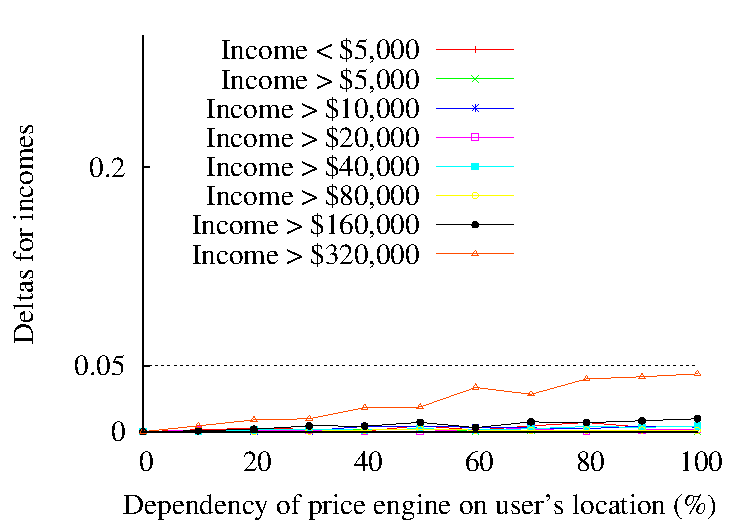
\includegraphics[width=0.33\textwidth]
    {\detokenize{results/income_discrimination_on_location_dependency}}
    \label{fig:DeltasIncome}
 }
 \subfigure[Race]{
    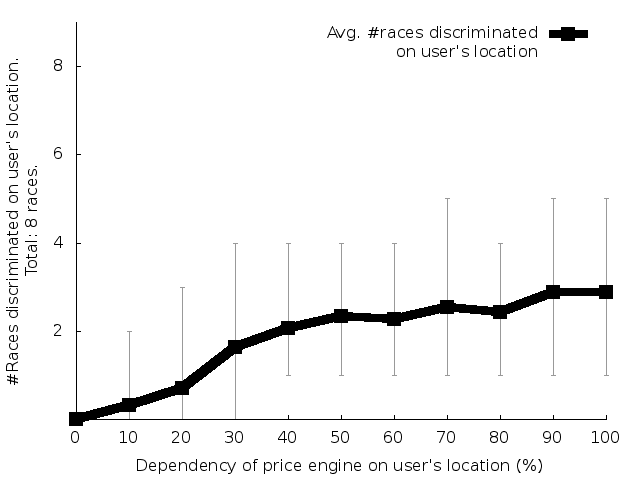
\includegraphics[width=0.33\textwidth]
    {\detokenize{results/race_discrimination_on_location_dependency}}
    \label{fig:DeltasRace}
  }
 \subfigure[Sex]{
    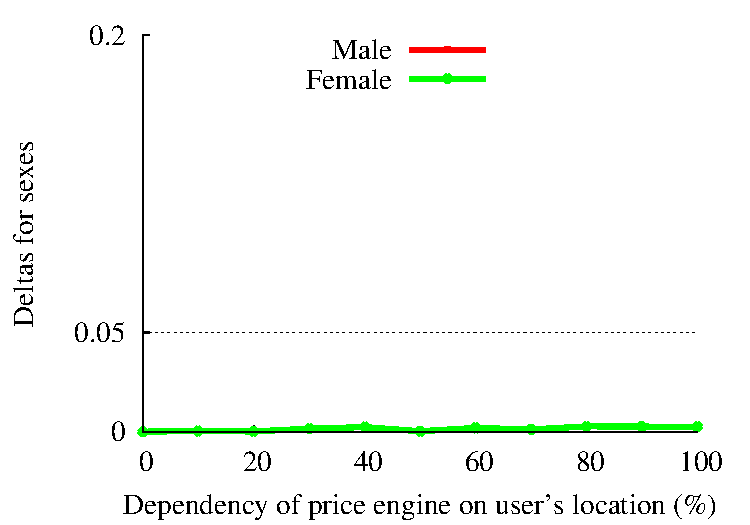
\includegraphics[width=0.33\textwidth]
    {\detokenize{results/sex_discrimination_on_location_dependency}}
    \label{fig:DeltasSex}
  }
 \caption{\textbf{Statistical parity and its dependency on user's location.}
          Shows the dependency of statistical parity, i.e., number of samples that
          violate condition~\ref{eq:StatisticalParity}, as a function of (a) user's income,
          (b) user's race, and (c) user's sex. Figure (b) reveals that statistical parity on
          user-incomes correlates with the dependency of the price engine on user's location.
          While Figures (a) and (b) reveal that statistical parity on user-race and on user-sex
          do not correlate with the dependency of the price engine on user's location.}
 \label{fig:Deltas}
}
\end{figure*}


\begin{figure*}[t]
{
 \subfigure[Race]{
    \includegraphics[width=0.33\textwidth]
    {\detokenize{results/income_discrimination_on_proportional}}
    \label{fig:}
  }
  \subfigure[Income]{
    \includegraphics[width=0.33\textwidth]
    {\detokenize{results/race_discrimination_on_proportional}}
    \label{fig:IncomeDiscriminationProportional}
 }
 \subfigure[Sex]{
    \includegraphics[width=0.33\textwidth]
    {\detokenize{results/sex_discrimination_on_proportional}}
    \label{fig:}
  }
 \caption{\textbf{Prices shown to users and their dependency on income, race, and sex.}
          Shows the proportion of high versus low prices shown to users based on income,
          race, and sex. Figure (b) reveals that a users with annual income less than
          \$5,000 receive proportionaly more high prices than users with annual income
          more than \$320,000. Figure (a) indicates that Indian or Alaskan users receive
          notably more high prices than any other race. This raises a consern, since as
          shown in Figure~\ref{fig:IncomePerRace}, an Indian or Alaskan user has a
          considerably lower income than a white American user. Figure (c) shows that
          male and female users receive approximately the same proportion of high versus
          low prices.}
}
\end{figure*}


\begin{figure}[!h]
 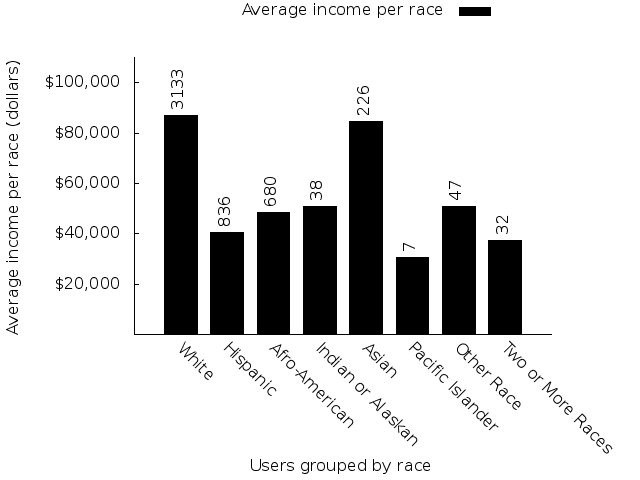
\includegraphics[width=0.49\textwidth]
  {\detokenize{results/income_per_race}}
  \caption{\textbf{Average user income for each race.} An Indian or Alaskan user has
           a considerably lower income than a white American user, and yet, as shown in
           Figure~\ref{fig:IncomeDiscriminationProportional}, he or she receives
           proportional more high prices compared to a white American.}
  \label{fig:IncomePerRace}
\end{figure}

\begin{figure*}[t]
{
 \subfigure[Race]{
    \includegraphics[width=0.33\textwidth]
    {\detokenize{results/misc/race_discrimination_on_proportional}}
    \label{fig:}
  }
  \subfigure[Income]{
    \includegraphics[width=0.33\textwidth]
    {\detokenize{results/misc/income_discrimination_on_proportional}}
    \label{fig:IncomeDiscriminationProportional}
 }
 \subfigure[Sex]{
    \includegraphics[width=0.33\textwidth]
    {\detokenize{results/misc/sex_discrimination_on_proportional}}
    \label{fig:}
  }
 \caption{\textbf{NEW:Prices shown to users and their dependency on income, race, and sex.}
          Shows the proportion of high versus low prices shown to users based on income,
          race, and sex. Figure (b) reveals that a users with annual income less than
          \$5,000 receive proportionaly more high prices than users with annual income
          more than \$320,000. Figure (a) indicates that Indian or Alaskan users receive
          notably more high prices than any other race. This raises a consern, since as
          shown in Figure~\ref{fig:IncomePerRace}, an Indian or Alaskan user has a
          considerably lower income than a white American user. Figure (c) shows that
          male and female users receive approximately the same proportion of high versus
          low prices.}
}
\end{figure*}



